% =====================================================================
% ARCH7476 · Evidence-Based Generative Design — Course Introduction Deck
% Tool Pathways for Studio Decisions
%
% Build:  xelatex course-intro.tex   (run twice for the progress bar)
% Needs:  TeX Live w/ metropolis theme; images resolved via ../assets
% Length: 18 frames ≈ 12–18 minutes
% =====================================================================
\documentclass[aspectratio=169,10pt]{beamer}
\usetheme[progressbar=frametitle,numbering=fraction]{metropolis}

% ---- fonts: Fira OTFs resolve from the TeX tree by filename (kpathsea),
% so no hardcoded path is needed. metropolis' own Fira lookup fails on macOS
% (it searches system font names) — its "Could not find Fira" warning is
% expected and harmless; we load the fonts ourselves below.
\setsansfont[
  Extension=.otf,
  UprightFont=FiraSans-Light,
  BoldFont=FiraSans-SemiBold,
  ItalicFont=FiraSans-LightItalic,
  BoldItalicFont=FiraSans-SemiBoldItalic]{FiraSans}
\setmonofont[
  Extension=.otf,
  UprightFont=FiraMono-Regular,
  BoldFont=FiraMono-Bold]{FiraMono}
% CJK face for the Kai Tak photo credit; degrade gracefully off-macOS
\IfFontExistsTF{PingFang HK}
  {\newfontfamily\cjkfont{PingFang HK}}
  {\IfFontExistsTF{Noto Sans CJK HK}
    {\newfontfamily\cjkfont{Noto Sans CJK HK}}
    {\let\cjkfont\sffamily}}

% ---- palette: ink + oxide accent; one muted hue per pathway
\definecolor{cInk}{HTML}{23373B}      % ink (frame titles, structure)
\definecolor{cAccent}{HTML}{C34A2C}   % oxide red (alerts, progress bar)
\definecolor{cSheet}{HTML}{2F6577}    % spreadsheet — slate teal
\definecolor{cGIS}{HTML}{5E7D3C}      % GIS — moss green
\definecolor{cPy}{HTML}{B0552F}       % python — sienna
\definecolor{cPaper}{HTML}{FAFAF8}    % background
\definecolor{cMute}{HTML}{596264}     % secondary text

\setbeamercolor{normal text}{fg=cInk,bg=cPaper}
\setbeamercolor{frametitle}{bg=cInk,fg=cPaper}
\setbeamercolor{progress bar}{fg=cAccent,bg=cInk!15}
\setbeamercolor{alerted text}{fg=cAccent}
\setbeamerfont{frametitle}{series=\bfseries,size=\large}
\setbeamerfont{title}{series=\bfseries}
\usepackage{array}

\usepackage{tikz}
\usetikzlibrary{positioning,arrows.meta,calc}
\usepackage[export]{adjustbox}
\usepackage{booktabs}
\usepackage{tcolorbox}
\tcbuselibrary{skins}

\graphicspath{{../}}   % deck lives in slides/, assets resolve from repo root

% ---- helpers ---------------------------------------------------------
\newcommand{\credit}[1]{{\tiny\color{cMute}#1\par}}
\newcommand{\muted}[1]{{\color{cMute}#1}}

% pathway card: thin colored left rule, quiet fill, sharp corners
\newtcolorbox{pathcard}[2]{enhanced,sharp corners,frame hidden,
  borderline west={2.5pt}{0pt}{#1},colback=cInk!4,
  boxsep=3pt,left=6pt,right=3pt,top=2pt,bottom=2pt,halign=left,
  title={\textbf{\color{#1}#2}},coltitle=cInk,
  attach title to upper={\par\vspace{2pt}}}

% case photos, cropped to a shared 1.555 aspect so grids sit flush
\newcommand{\imgEdge}[1]{\adjincludegraphics[width=#1,trim={0 {.136\height} 0 {.06\height}},clip]{assets/examples/the-edge-amsterdam.jpg}}
\newcommand{\imgHighline}[1]{\adjincludegraphics[width=#1,trim={0 {.04\height} 0 {.03\height}},clip]{assets/examples/high-line-park.jpg}}
\newcommand{\imgCalac}[1]{\adjincludegraphics[width=#1,trim={{.0625\width} 0 {.0625\width} 0},clip]{assets/examples/california-academy-of-sciences.jpg}}
\newcommand{\imgKaitak}[1]{\adjincludegraphics[width=#1,trim={0 {.063\height} 0 {.08\height}},clip]{assets/examples/kai-tak-sports-park.jpg}}

\title{Evidence-Based Generative Design}
\subtitle{Tool Pathways for Studio Decisions}
\author{Hongshan Guo}
\institute{Department of Architecture · The University of Hong Kong}
\date{}

\begin{document}

% =====================================================================
\begin{frame}[plain]
  \vspace{3mm}
  {\color{cMute}\small ARCH7476 · Department of Architecture · The University of Hong Kong}\par
  \vspace{3mm}
  {\Huge\bfseries Evidence-Based\\Generative Design}\par
  \vspace{2mm}
  {\Large\color{cAccent} Tool Pathways for Studio Decisions}\par
  \vspace{1.5mm}
  {\small\muted{\itshape Generate comparable options, not renders --- with a workflow you keep.}}\par
  \vspace{2mm}
  {\color{cInk}Hongshan Guo}\quad\muted{·}\quad
  \muted{12 weeks × 2 hours}\quad\muted{·}\quad
  \muted{undergraduate, MArch, and PhD in one room}
  \vfill
  \begin{columns}[T]
    \column{.245\textwidth}\imgEdge{\textwidth}
    \column{.245\textwidth}\imgHighline{\textwidth}
    \column{.245\textwidth}\imgCalac{\textwidth}
    \column{.245\textwidth}\imgKaitak{\textwidth}
  \end{columns}
  \vspace{1mm}
  \credit{Photos: AValečka · Dansnguyen · Dennis G. Jarvis · {\cjkfont 建園春秋} --- CC, via Wikimedia Commons (full credits with the case gallery)}
\end{frame}

% =====================================================================
\begin{frame}{One question runs the whole semester}
  Final review. ``The atrium improves daylight.''
  A critic asks: \alert{by how much? compared to what?}
  \vspace{1.5mm}
  \begin{center}
    {\LARGE\itshape What evidence would make this design\\decision more defensible?}
  \end{center}
  \vspace{1.5mm}
  Where studio decisions usually come from — all of us, no exceptions:
  \begin{itemize}
    \item precedent and intuition · tutor pressure, or taste
    \item assumptions nobody tested · ``evidence'' added after the decision,
          to justify it
  \end{itemize}
  \vspace{1mm}
  \alert{The reframe:} not \emph{``what software should I use?''} but
  \emph{``what evidence would reduce uncertainty around \textbf{this}
  decision?''} --- and then the shortest workflow that produces it.
\end{frame}

% =====================================================================
\begin{frame}{Straight talk: this is not last year's course}
  Last year's feedback was clear --- too philosophical, not useful enough.
  We rebuilt the semester around the tools.
  \vspace{1.5mm}

  \footnotesize
  \begin{tabular}{@{}p{.44\textwidth}@{\hspace{6mm}}p{.48\textwidth}@{}}
    \muted{\textbf{Was}} & \textbf{Is now}\\
    \midrule
    course philosophy first & tool landscape first --- week 1 is a working session\\
    a ``research brief'' to write & a studio decision you actually face\\
    theory readings & named drills, every single week\\
    two loose tracks (no/low-code vs code-heavy) & \textbf{one assessed pathway you choose:} \textcolor{cSheet}{\textbf{Spreadsheet}}, \textcolor{cGIS}{\textbf{GIS}}, or \textcolor{cPy}{\textbf{Python}}\\
    a machine-learning theory detour & Python = notebooks you adapt; ML strictly optional\\
    first working build due wk 5 & first working build due wk 8 --- real time to build\\
  \end{tabular}

  \vspace{2.5mm}
  \small
  What we kept: the four-assignment arc and its weights, mentor
  consultations, and the week-12 \alert{Object Fair}.
\end{frame}

% =====================================================================
\begin{frame}{How you will actually generate}
  \vspace{-1mm}
  \begin{center}
  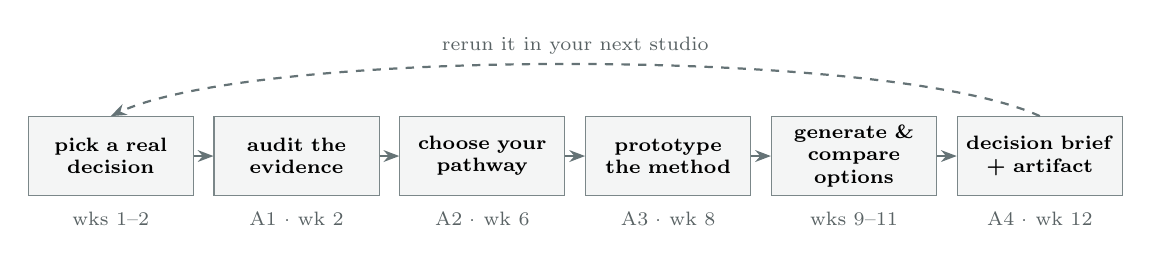
\begin{tikzpicture}[
      stp/.style={draw=cInk!60,fill=cInk!5,text width=19.2mm,align=center,
                   inner sep=2.5pt,minimum height=10mm,font=\scriptsize},
      wk/.style={font=\scriptsize,color=cMute},
      arr/.style={-{Stealth[length=2mm]},thick,color=cInk!70}]
    \node[stp] (a) {\textbf{pick a real}\\\textbf{decision}};
    \node[stp,right=2.5mm of a] (b) {\textbf{audit the}\\\textbf{evidence}};
    \node[stp,right=2.5mm of b] (c) {\textbf{choose your}\\\textbf{pathway}};
    \node[stp,right=2.5mm of c] (d) {\textbf{prototype}\\\textbf{the method}};
    \node[stp,right=2.5mm of d] (e) {\textbf{generate \&}\\\textbf{compare options}};
    \node[stp,right=2.5mm of e] (f) {\textbf{decision brief}\\\textbf{+ artifact}};
    \draw[arr] (a) -- (b); \draw[arr] (b) -- (c); \draw[arr] (c) -- (d);
    \draw[arr] (d) -- (e); \draw[arr] (e) -- (f);
    \node[wk,below=.8mm of a] {wks 1--2};
    \node[wk,below=.8mm of b] {A1 · wk 2};
    \node[wk,below=.8mm of c] {A2 · wk 6};
    \node[wk,below=.8mm of d] {A3 · wk 8};
    \node[wk,below=.8mm of e] {wks 9--11};
    \node[wk,below=.8mm of f] {A4 · wk 12};
    \draw[arr,dashed,looseness=.45] (f.north) to[out=155,in=25]
      node[above,font=\scriptsize,color=cMute]{rerun it in your next studio} (a.north);
  \end{tikzpicture}
  \end{center}
  Generating means producing \emph{comparable options}, not renders:
  \begin{itemize}
    \item \textcolor{cSheet}{\textbf{Spreadsheet}} — score options A/B/C on daylight, access, cost, risk \(\rightarrow\) a decision matrix
    \item \textcolor{cGIS}{\textbf{GIS}} — three candidate sites × 400\,m buffers and walksheds \(\rightarrow\) a defensible site pick
    \item \textcolor{cPy}{\textbf{Python}} — 200 design variants \(\rightarrow\) cooling, daylight, and glare trade-off charts \muted{(dataset provided, or your own variant sweep --- you write the analysis)}
  \end{itemize}
  \alert{``Generative'' here is a workflow you can rerun --- evidence in, defensible options out.}
\end{frame}

% =====================================================================
\begin{frame}{Choose one pathway --- go deep, keep the others legible}
  \begin{columns}[T]
    \column{.32\textwidth}
    \begin{pathcard}{cSheet}{SPREADSHEET}
      \scriptsize Excel · Google Sheets\\[2pt]
      Best when the decision needs \textbf{comparison, ranking,
      visible logic}.\\[2pt]
      You build: evidence log \(\rightarrow\) alternatives \(\rightarrow\)
      charts with ranges \(\rightarrow\) decision matrix.\\[2pt]
      \muted{The baseline exit pathway. Not remedial --- the
      lowest-friction route to a decision-ready workflow.}
    \end{pathcard}
    \column{.32\textwidth}
    \begin{pathcard}{cGIS}{GIS}
      \scriptsize QGIS · ArcGIS · geopandas\\[2pt]
      Best when \textbf{site, access, zoning, or overlap} drives
      the decision.\\[2pt]
      You build: buffers, walksheds, spatial joins \(\rightarrow\) one clean
      map per question.\\[2pt]
      \muted{Week 4 compares all three head-to-head --- and these are the
      outputs feasibility and masterplanning teams actually use.}
    \end{pathcard}
    \column{.32\textwidth}
    \begin{pathcard}{cPy}{PYTHON}
      \scriptsize Jupyter · pandas · Colab\\[2pt]
      Best when \textbf{repeatability, reuse, or scale}
      matters.\\[2pt]
      You build: notebook analyses adapted from the course starters ---
      never \emph{required} to start from a blank file.\\[2pt]
      \muted{``If a spreadsheet answers the question cleanly,
      that is still a strong choice.''}
    \end{pathcard}
  \end{columns}
  \vspace{1.5mm}
  \footnotesize
  The week-6 commitment test --- if you cannot finish this sentence, you have
  not chosen yet: \emph{``I am choosing \_\_\_ because my decision depends
  primarily on \_\_\_, and the minimum useful output will be \_\_\_.''}\par
  \vspace{.8mm}
  \alert{Pathway choice should feel boring:} the shortest path to a useful
  output --- never the most impressive tool.
\end{frame}

% =====================================================================
\begin{frame}{BIM, BEM, performance: literacy for everyone, pathway for no one}
  \begin{itemize}
    \item \textbf{BIM} answers \emph{what do we build and how does it fit together};
          \textbf{BEM} answers \emph{how will it behave over time}
    \item translation between them loses geometry, zones, constructions,
          operations --- \alert{translation loss is normal, not an edge case}
    \item simulation is evidence --- useful, never automatically authoritative
    \item the paired-run rule: simulate your variants A and B --- the
          \emph{delta} outlives translation error
  \end{itemize}
  \vspace{.5mm}
  \begin{tcolorbox}[enhanced,sharp corners,frame hidden,colback=cInk!5,
    borderline west={2.5pt}{0pt}{cAccent},boxsep=3pt,left=6pt]
    \footnotesize\textbf{Week 5 drill --- Translation Detective.} A five-storey
    office exports to gbXML (the standard BIM\(\rightarrow\)energy-model
    handoff) and reports \textbf{3× the expected energy use}. Your team finds
    the failure before anyone trusts the number. The week's real-scale case:
    \textbf{465 thermal zones} where \(\sim\)30 belong.
  \end{tcolorbox}
  \vspace{1mm}
  The week's lesson: \emph{``The file opened'' did not mean ``the model is
  valid.''}\par
  \muted{Taught to everyone --- but your assessed pathway stays Spreadsheet,
  GIS, or Python.}
\end{frame}

% =====================================================================
\begin{frame}{Four buildings we keep interrogating}
  These four recur all semester as standing prompts: \emph{what evidence would
  you want before defending this claim in public?}
  \vspace{2.5mm}

  \begin{columns}[T]
    \column{.235\textwidth}
    \imgEdge{\textwidth}\par\vspace{1mm}
    {\scriptsize\textbf{The Edge}\\Amsterdam\par\vspace{.5mm}
    \muted{wk 11 review lens: performance claim --- method, or branding?}}
    \column{.235\textwidth}
    \imgHighline{\textwidth}\par\vspace{1mm}
    {\scriptsize\textbf{High Line}\\New York\par\vspace{.5mm}
    \muted{wk 3: what would your spreadsheet need to track?}}
    \column{.235\textwidth}
    \imgCalac{\textwidth}\par\vspace{1mm}
    {\scriptsize\textbf{California Academy of Sciences}\\San Francisco\par\vspace{.5mm}
    \muted{wk 5: what evidence backs the envelope claim?}}
    \column{.235\textwidth}
    \imgKaitak{\textwidth}\par\vspace{1mm}
    {\scriptsize\textbf{Kai Tak Sports Park}\\Hong Kong\par\vspace{.5mm}
    \muted{wks 4 + 6: the local site, access, and urban evidence case}}
  \end{columns}
  \vfill
  \credit{AValečka CC BY-SA 4.0 · Dansnguyen CC0 · Dennis G. Jarvis CC BY-SA 2.0 · {\cjkfont 建園春秋} CC BY-SA 4.0 (photographed during construction, 2024) — via Wikimedia Commons}
\end{frame}

% =====================================================================
\begin{frame}{Twelve weeks, three phases, four deadlines}
  \begin{center}
  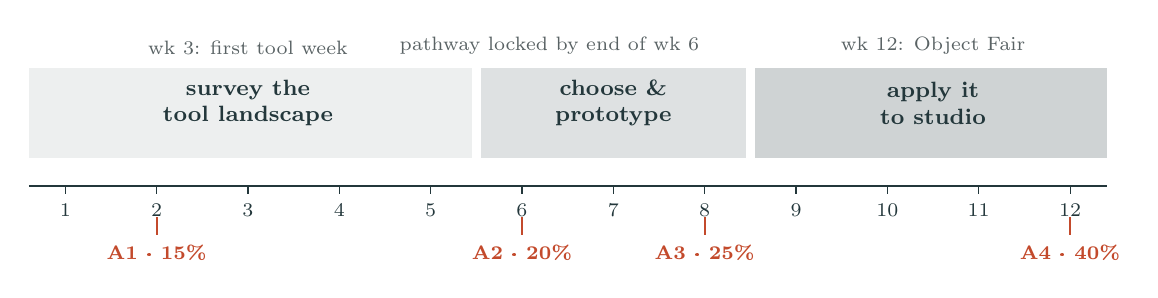
\begin{tikzpicture}[x=11.6mm,
      flag/.style={font=\scriptsize\bfseries,color=cAccent},
      wknum/.style={font=\scriptsize,color=cInk},
      phase/.style={font=\footnotesize\bfseries,align=center}]
    % phase bands (neutral tints — teal/moss/sienna stay reserved for pathways)
    \fill[cInk!8]  (0.6,0.35) rectangle (5.45,1.5);
    \fill[cInk!15] (5.55,0.35) rectangle (8.45,1.5);
    \fill[cInk!22] (8.55,0.35) rectangle (12.4,1.5);
    \node[phase,color=cInk] at (3.0,1.05) {survey the\\tool landscape};
    \node[phase,color=cInk] at (7.0,1.05) {choose \&\\prototype};
    \node[phase,color=cInk] at (10.5,1.05){apply it\\to studio};
    % axis + week ticks
    \draw[thick,color=cInk] (0.6,0) -- (12.4,0);
    \foreach \w in {1,...,12} {
      \draw[color=cInk] (\w,0) -- (\w,-0.1);
      \node[wknum,below=1mm] at (\w,0) {\w};
    }
    % assignment flags
    \foreach \w/\a/\p in {2/A1/15\%, 6/A2/20\%, 8/A3/25\%, 12/A4/40\%} {
      \draw[color=cAccent,thick] (\w,-0.62) -- (\w,-0.40);
      \node[flag,below] at (\w,-0.62) {\a\ · \p};
    }
    % milestones
    \node[font=\scriptsize,color=cMute,above] at (3,1.55) {wk 3: first tool week};
    \node[font=\scriptsize,color=cMute,above] at (6.3,1.55) {pathway locked by end of wk 6};
    \node[font=\scriptsize,color=cMute,above] at (10.5,1.55) {wk 12: Object Fair};
  \end{tikzpicture}
  \end{center}
  \vspace{3mm}
  \begin{itemize}
    \item \textbf{weeks 1--5} — audit your own evidence, then survey spreadsheet,
          GIS, and BIM/BEM literacy with drills each week
    \item \textbf{weeks 6--8} — commit to one pathway, build and pilot the
          smallest workflow that answers a real piece of your question
    \item \textbf{weeks 9--12} — figures, thresholds, a structured draft
          review, and a public Object Fair with critique
  \end{itemize}
\end{frame}

% =====================================================================
\begin{frame}{You make things in class --- every week}
  \footnotesize
  \begin{tabular}{@{}c@{\hspace{4mm}}p{.88\textwidth}@{}}
    \muted{wk} & \\
    \midrule
    1 & sort your own past evidence --- measured, observed, simulated, cited,
        tested by making, assumed --- and leave with \textbf{A1 already
        underway}\\
    2 & turn one prior decision into a full evidence audit; \muted{A1 due}\\
    3 & 15-minute \textbf{Workbook Build Sprint} on your own topic, then the
        \textbf{Peer Swap Test} --- can a classmate read your logic?\\
    4 & \textbf{Tool Choice Drill} (QGIS vs ArcGIS vs geopandas) + a live
        geopandas demo: load, inspect CRS, filter, buffer, plot, export\\
    5 & \textbf{Translation Detective} --- diagnose a BIM\(\rightarrow\)BEM
        export before trusting its numbers\\
    6 & \textbf{Pathway Commitment Drill} + in-class A2 work session;
        \muted{A2 due}\\
    7 & \textbf{10-Minute Method Challenge} + \textbf{Documentation Swap}
        across pathways, no verbal explanation allowed\\
    8 & pilot your method; upgrade the language: \emph{``the pilot suggests''},
        never \emph{``the data proves''}; \muted{A3 due}\\
    9 & \textbf{Figure Rescue Sprint} + \textbf{Option B Drill} --- the
        3-second test; your variants count as evidence\\
    10 & \textbf{draft review} --- pressure-test the near-final package,
        leave with a revision plan\\
    11 & \textbf{Evidence Package Workshop} --- peer review against four
        questions before anything is final\\
    12 & \textbf{Object Fair} --- public pin-up: your evidence board, your
        recommendation, your limits; \muted{A4 due}\\
  \end{tabular}
\end{frame}

% =====================================================================
\begin{frame}{Four assignments, one thread: a decision you actually face}
  \small
  \begin{tabular}{@{}p{.40\textwidth}ccp{.33\textwidth}@{}}
    & \muted{due} & \muted{weight} & \muted{the question it answers}\\
    \midrule
    \textbf{A1} Evidence Audit + Next Decision Brief & wk 2 & 15\% &
      what did I really know --- and what do I need next?\\[.5mm]
    \textbf{A2} Evidence and Pathway Map & wk 6 & 20\% &
      which sources, which workflow, and why?\\[.5mm]
    \textbf{A3} Method Prototype & wk 8 & 25\% &
      can I run a credible pilot in my pathway?\\[.5mm]
    \textbf{A4} Studio Evidence Package & wk 12 & 40\% &
      can someone act on this?\\
  \end{tabular}
  \vspace{2mm}

  \begin{itemize}
    \item each assignment builds directly on the previous one --- same project,
          rising stakes
    \item A3's standard: \emph{``The purpose is not scale. The purpose is
          proof''} that your pathway can produce decision-relevant output ---
          a working artifact that is \alert{interpretable, not polished}
    \item no exams, no quizzes --- the four assignments are 100\% of the
          grade, \(\approx\)50--70 hours outside class all semester; drills
          are practice, not graded, but they build your assignment material
  \end{itemize}
\end{frame}

% =====================================================================
\begin{frame}{Where it lands: the Object Fair, week 12}
  \textbf{A4 --- the Studio Evidence Package (40\%)} has four parts that
  reinforce each other:
  \begin{enumerate}
    \item a \textbf{studio decision brief} (6--10 pages, written for critics
          and practice stakeholders)
    \item an \textbf{evidence board / object card} --- one poster-scale page
          that survives 30 seconds of a stranger's attention
    \item the \textbf{pathway artifact} --- your working workbook, map set, or
          notebook; \muted{it proves the package came from a workflow, not
          from slides}
    \item a \textbf{method appendix} (2--4 pages) --- enough for someone else
          to rerun or extend the work
  \end{enumerate}
  \vspace{2mm}
  At the fair you present five things:
  \begin{center}
    \textbf{the decision · the pathway · the evidence · the recommendation · the limit}
  \end{center}
  \vspace{1mm}
  This is not just a report. It is a decision-support package --- and it is
  yours to reuse.
\end{frame}

% =====================================================================
\begin{frame}{The standard for evidence: ranges, not single numbers}
  \begin{center}
    \adjincludegraphics[width=.63\textwidth,trim={0 {.14\height} 0 0},clip]{assets/02MC.png}
  \end{center}
  \vspace{.5mm}
  {\scriptsize One room, two claims of very different strength: PMV
  (the standard single-number comfort score) vs.\ the predicted
  \emph{distribution} of what occupants actually feel.
  \muted{(Figure from the instructor's research.)}\par}
  \vspace{.5mm}
  \begin{itemize}
    \item every pathway ends the same way: \textbf{uncertainty shown, not
          hidden} --- ranges on key figures are in the A4 rubric, and
          transparency about limits is 25\% of A3
    \item \textcolor{cSheet}{scenario bands} in the workbook ·
          \textcolor{cGIS}{stated extents and assumptions} on the map ·
          \textcolor{cPy}{confidence intervals} in the notebook
  \end{itemize}
\end{frame}

% =====================================================================
\begin{frame}{You do not start from zero}
  \footnotesize
  \begin{columns}[T]
    \column{.52\textwidth}
    {\small\textbf{In the repo on day one}}
    \begin{itemize}
      \item \textbf{starter notebooks} you adapt --- you never have to start
            blank: an A/B pilot analysis with error bars and an object-card
            starter figure, plus an optional modeling extension
      \item \textbf{three practice datasets}, openly synthetic: 200 design
            variants (cooling / daylight / glare), a 120-row A/B pilot log,
            and 60 occupant survey comments --- swap in your own data with
            the same structure
      \item the four-image precedent bank, licensing already sorted
    \end{itemize}
    \column{.44\textwidth}
    {\small\textbf{Setup ladder}}
    \begin{itemize}
      \item \emph{``use the lightest setup that still lets you complete your
            chosen pathway well''}
      \item spreadsheet access --- everyone
      \item QGIS --- only if you choose GIS
      \item Anaconda + Jupyter --- only for Python or code-based GIS
            (geopandas); \textbf{Colab} is the no-install fallback
    \end{itemize}
    {\small\textbf{Local data that is actually there}}\\
    DATA.GOV.HK, Planning \& Transport Departments,
    HK Observatory climate records, OpenStreetMap\par
  \end{columns}
  \vspace{1.5mm}
  \small\textbf{Humans:} office hours (setup + pathway troubleshooting) ·
  in-class work sessions · peer review
\end{frame}

% =====================================================================
\begin{frame}{The takeaways are explicit --- and they are tools}
  The syllabus states five learning outcomes; this is the form you actually
  hold them in by week 12:
  \begin{enumerate}
    \item a \textbf{working workflow artifact} in your pathway --- workbook,
          map set, or notebook --- built on your own project, reusable in the
          next one
    \item an \textbf{evidence audit habit}: measured / observed / simulated /
          cited / tested by making / assumed --- applied before the decision,
          not after
    \item \textbf{judgment about tool fit} --- when a spreadsheet beats a
          notebook, when a map beats both
    \item a \textbf{language for uncertainty and thresholds} that critics and
          clients take seriously
    \item a \textbf{documented method} someone else could rerun --- your
          method appendix
  \end{enumerate}
  \vspace{3mm}
  The closing standard: strong work never sounds like \emph{``I used a tool.''}\\
  It sounds like \alert{``I used this workflow to reduce uncertainty around a
  real design decision.''}
\end{frame}

% =====================================================================
\begin{frame}{What is graded --- and what deliberately is not}
  \begin{columns}[T]
    \column{.485\textwidth}
    \textbf{Graded, in every rubric}
    \begin{itemize}
      \item method--question \textbf{fit}
      \item \textbf{honesty}: A1 grades specificity \& honesty at 35\%;
            A3 grades transparency about limits at 25\%
      \item a workflow that can be \textbf{rerun or explained}
      \item \textbf{decision usefulness} --- could a stakeholder act on it?
    \end{itemize}
    \column{.485\textwidth}
    \textbf{\muted{Not graded, ever}}
    \begin{itemize}
      \item tool virtuosity or code elegance
      \item how many software packages you touched
      \item choosing the most intimidating tool ---
            \emph{``overreach''} means a tool the question doesn't need,
            never depth within one it does
    \end{itemize}
  \end{columns}
  \vspace{2.5mm}
  \alert{The tools are takeaways, not the graded object.} Support is scoped to
  your one pathway --- starter files, a setup ladder, office hours, peer
  swaps; we don't train you across all three tools. Tiers are floors, not
  ceilings: opting into deeper expectations is never a grade risk. This is a
  course in deciding with evidence, not software training.
\end{frame}

% =====================================================================
\begin{frame}{What this course is not}
  Worth knowing before pathways lock in week 6 --- this course is \textbf{not}:
  \begin{itemize}
    \item \textbf{software training} --- no feature tours, no certification;
          the deepest \emph{required} code is a five-line geopandas workflow,
          the Spreadsheet pathway needs none, and the optional notebooks go
          further for anyone who wants depth
    \item \textbf{an AI/ML course} --- Python here means pandas and notebooks;
          machine learning is optional depth for those who want it
    \item \textbf{a theory seminar} --- no readings-driven weeks; every concept
          lives inside a drill, a template, or a rubric
    \item \textbf{a data-science conversion} --- you stay a designer: the
          tools serve design decisions, they don't replace them
  \end{itemize}
  \vspace{2mm}
  And honest pacing, so nobody is surprised: weeks 1--2 audit \emph{your own}
  past decisions (working sessions, not software demos); the first tool week
  is week 3; your first full build lands in weeks 7--8.
\end{frame}

% =====================================================================
\begin{frame}{Same arc for everyone --- depth scales}
  \small
  \begin{tabular}{@{}>{\raggedright\arraybackslash}p{.17\textwidth}>{\raggedright\arraybackslash}p{.36\textwidth}>{\raggedright\arraybackslash}p{.38\textwidth}@{}}
    & \muted{what stays common} & \muted{what scales}\\
    \midrule
    Undergraduate & same weeks, same four assignments & tighter scope, more scaffolding\\[1.5mm]
    \textbf{MArch} & \textbf{same weeks, same four assignments} &
      \textbf{stakeholder fit, independence, practice-ready outputs}\\[1.5mm]
    PhD & same weeks, same four assignments & deeper uncertainty treatment, stronger reproducibility\\
  \end{tabular}
  \vspace{4mm}

  \begin{itemize}
    \item the difference is \alert{depth and independence, not separate coursework}
    \item you are never rewarded for out-teching the room --- only for fitting
          the method to the question in front of you
  \end{itemize}
\end{frame}

% =====================================================================
\begin{frame}{Come to week 1 with three things}
  \begin{enumerate}
    \item \textbf{one design decision you already made} --- a façade
          proportion, an entrance location, a shading strategy --- plus
          whatever counted as evidence at the time
    \item \textbf{one upcoming studio decision} worth investigating --- a
          live thesis decision is explicitly welcome; the course runs
          alongside it
    \item \textbf{working spreadsheet access} --- Excel or Google Sheets,
          the whole week-1 setup
  \end{enumerate}
  \vspace{2mm}
  You will leave the first session with A1 already underway.
  \vspace{1mm}
  \begin{center}
    {\large\itshape By week 12 you should be able to say:}\\[2mm]
    {\large ``This is the decision, this is the evidence,\\
    this is the method --- and this is how confident I am.''}
  \end{center}
  \vfill
  Everything lives on the course site: schedule, assignment briefs, starter
  notebooks, and setup guides --- \muted{questions any time at office hours.}
\end{frame}

\end{document}
